\documentclass[twocolumn]{article}

\usepackage{graphicx} % Required for inserting images
\usepackage{amsmath}
\usepackage{amssymb}
\usepackage{url}
\usepackage[a4paper, left=1.5cm, right=1.5cm, top=2.5cm, bottom=2.5cm]{geometry}
\usepackage{etoolbox}
\usepackage{booktabs}
%\usepackage{svg}

\patchcmd{\thebibliography}{\section*{\refname}}{}{}{}

\title{Análisis de la Movilidad en la Zona Metropolitana del Valle de México con Redes Bayesianas}

\author{
Alan Fernando Bravo Pimentel \and
Gonzalo Makenly Higuera Inzunza \and
Juan Pablo de la Peña Gonzalez \and
Sarah Camila Guzmán Fierro}

\date{Agosto 2025}

\begin{document}

\maketitle

\begin{abstract}
En este estudio utilizamos datos de la \textit{Encuesta Origen Destino en Hogares} (EOD 2017), de la Zona Metropolitana del Valle de México (ZMVM) -recopilada por el Instituto Nacional de Estadística y Geografía (INEGI)-, para responder consultas probabilísticas relacionadas con el uso de transporte. El objetivo principal es comprender patrones dentro de los hábitos de transporte de la población ya sean socioeconómicos, por edad, o sexo. Se construyeron redes bayesianas a partir de las variables a observar, se propusieron tres estructuras iniciales de grafos dirigidos acíclicos (DAGs), y posteriormente se aplicó el algoritmo \textit{hill-climbing} para identificar la estructura con mejor ajuste. Los resultados muestran que los adultos presentan gran probabilidad de utilizar transporte ferroviario; el uso de transporte privado es más común en fin de semana que en días hábiles; los hombres adultos son poco propensos a usar automóvil por motivos de trabajo; y los individuos de estrato bajo tienen menor probabilidad de realizar viajes de más de 90 minutos de sus casas al trabajo.
\end{abstract}

\section{Introducción}
La movilidad urbana en la Zona Metropolitana del Valle de México (ZMVM) es un fenómeno complejo que involucra factores demográficos, socioeconómicos y de infraestructura. Para comprender mejor los patrones de transporte, el INEGI realizó en 2017 la \textit{Encuesta Origen Destino en Hogares}, cuyo objetivo fue obtener información que permita conocer la movilidad actual de los habitantes de la ZMVM. Este contiene bases de datos relacionadas mediante llaves, se pueden observar datos del viaje que tomó la persona encuestada, sus datos de patrimonio, localidad y estado de vivienda. Hay conteos similares como la Encuesta Anual del Transporte, igualmente sostenida por el INEGI, la Encuesta de Movilidad del Estado de México, Encuesta de Percepción de la Seguridad en el Transporte Público, así como estadísticos proporcionados por la Secretaria de Comunicaciones y Transportes; todos los cuales tienen como objetivo aportar conocimiento sobre la calidad y seguridad de la distribución de volumen vehicular.

En este trabajo utilizamos una aproximación basada en \textbf{redes bayesianas} para modelar las dependencias probabilísticas entre variables de interés, y responder consultas que permiten evaluar probabilidades condicionales asociadas al uso de transporte público o privado, duración de viajes y su relación con estrato socioeconómico, edad y sexo. Estos resultados tienen el propósito de provocar reflexión sobre las posibles ventajas o desventajas que pueda presentar un grupo demográfico.

\section{Metodología}
\begin{enumerate}
    \item \textbf{Selección y preparación de variables}: Se identificaron variables relevantes: edad, sexo, estrato socioeconómico, día de la semana (entre semana ó fin de semana), medio de transporte, tiempo, propósito y origen de viaje; localidad de origen. Variables continuas como edad y tiempo de viaje fueron discretizadas en categorías (\textit{Adulto/Menor} y \textit{Corto/Largo}).
      
    \item \textbf{Construcción de DAGs}: Se propusieron tres grafos dirigidos acíclicos (DAGs) con diferentes enfoques: construcción por intuición, con prioridad a la demografía y con prioridad al concepto de transporte. A su vez se calculó su \textit{Criterio de información bayesiano (BIC)} y la fuerza de los arcos.
    \begin{itemize}
        \item \textbf{DAG 1}: basada en sentido común. 
            \begin{figure}[htbp]
                \centering
                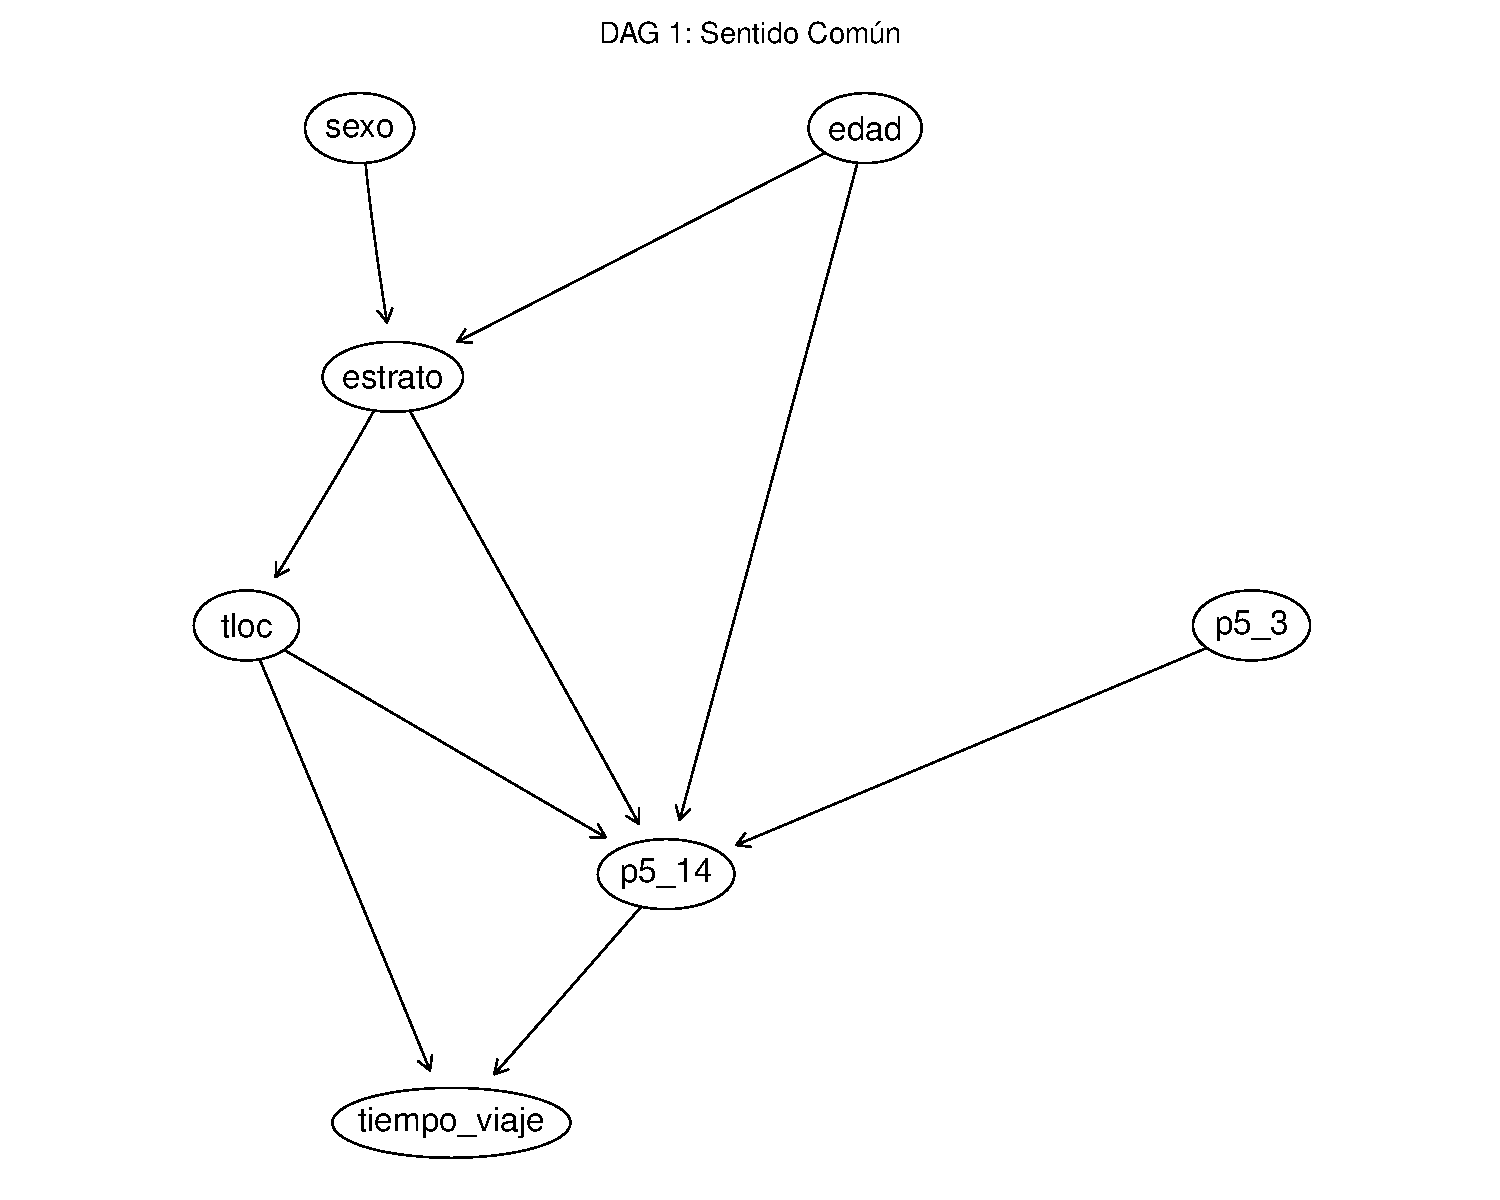
\includegraphics[width=0.8\columnwidth]{figures/DAG1_sentido_comun.pdf}
                \caption{DAG 1: Sentido Común}
                \label{fig:dag1}
            \end{figure}
            
            $BIC_1=-6327715$
        \item \textbf{DAG 2}: centrada en demografía. 
            \begin{figure}[htbp]
                \centering
                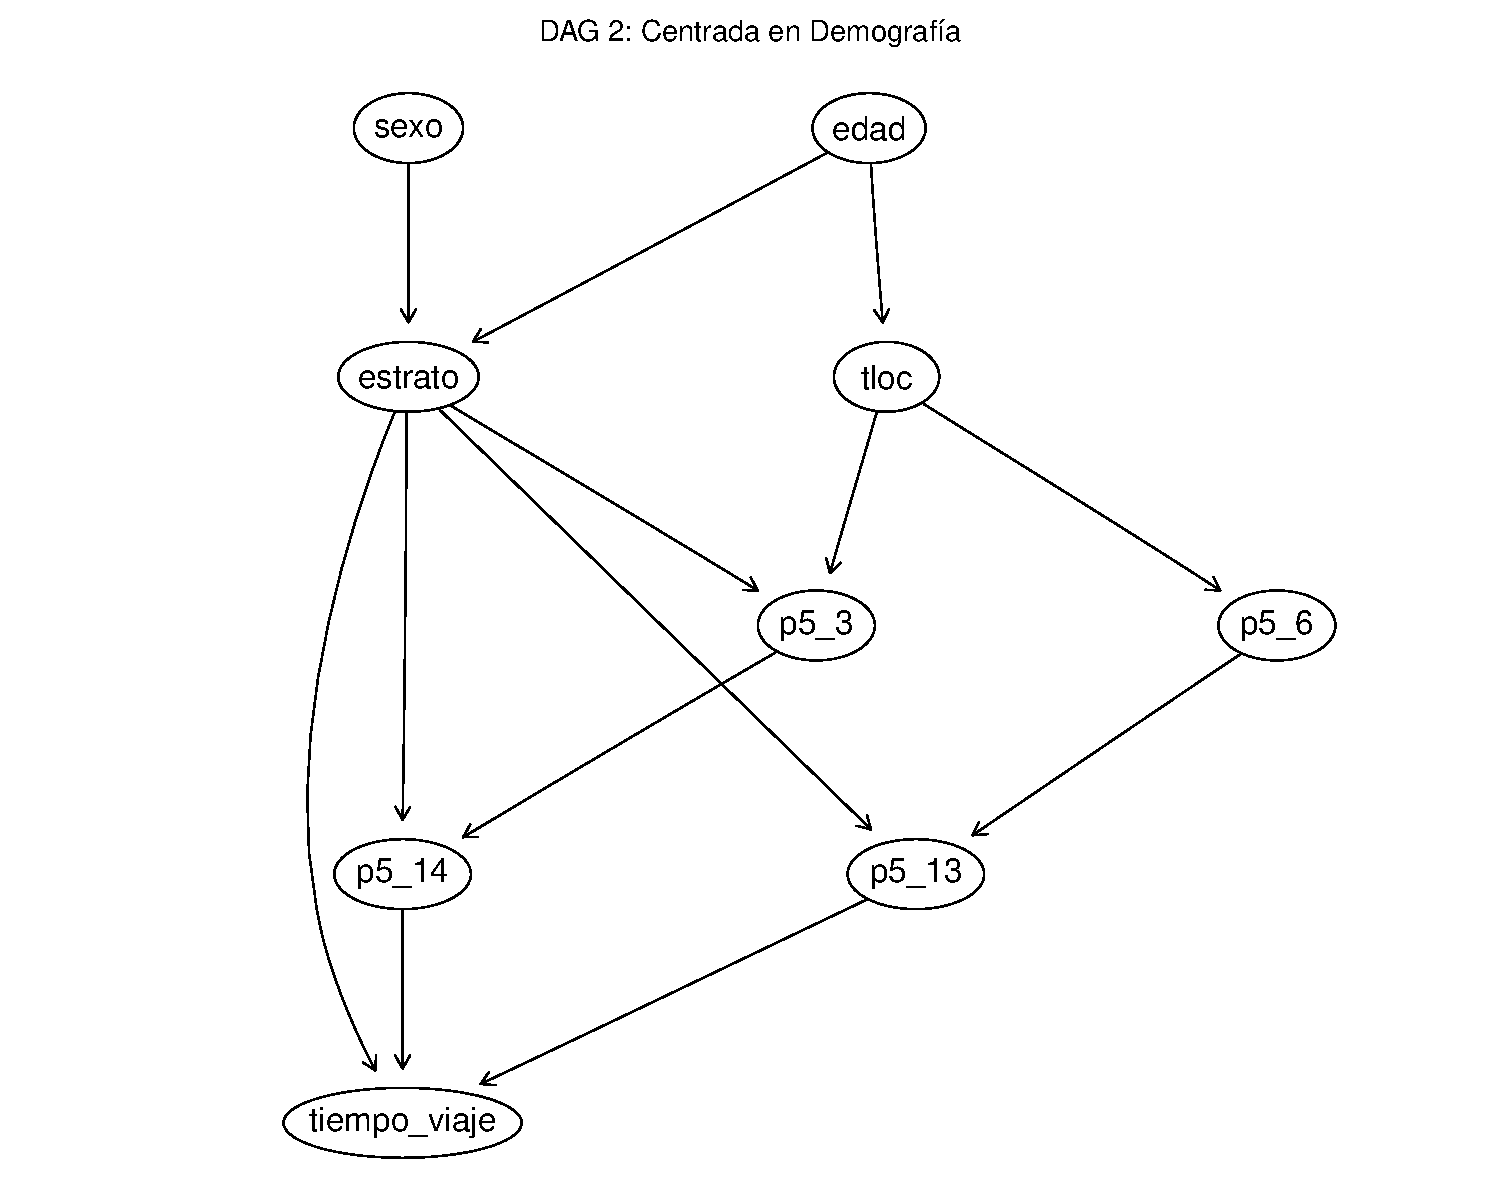
\includegraphics[width=0.8\columnwidth]{figures/DAG2_demografia.pdf}
                \caption{DAG 2: Demografía}
                \label{fig:dag2}
            \end{figure}
            
            $BIC_2=-6454501$
        \item \textbf{DAG 3}: centrada en transporte. 
            \begin{figure}[htbp]
                \centering
                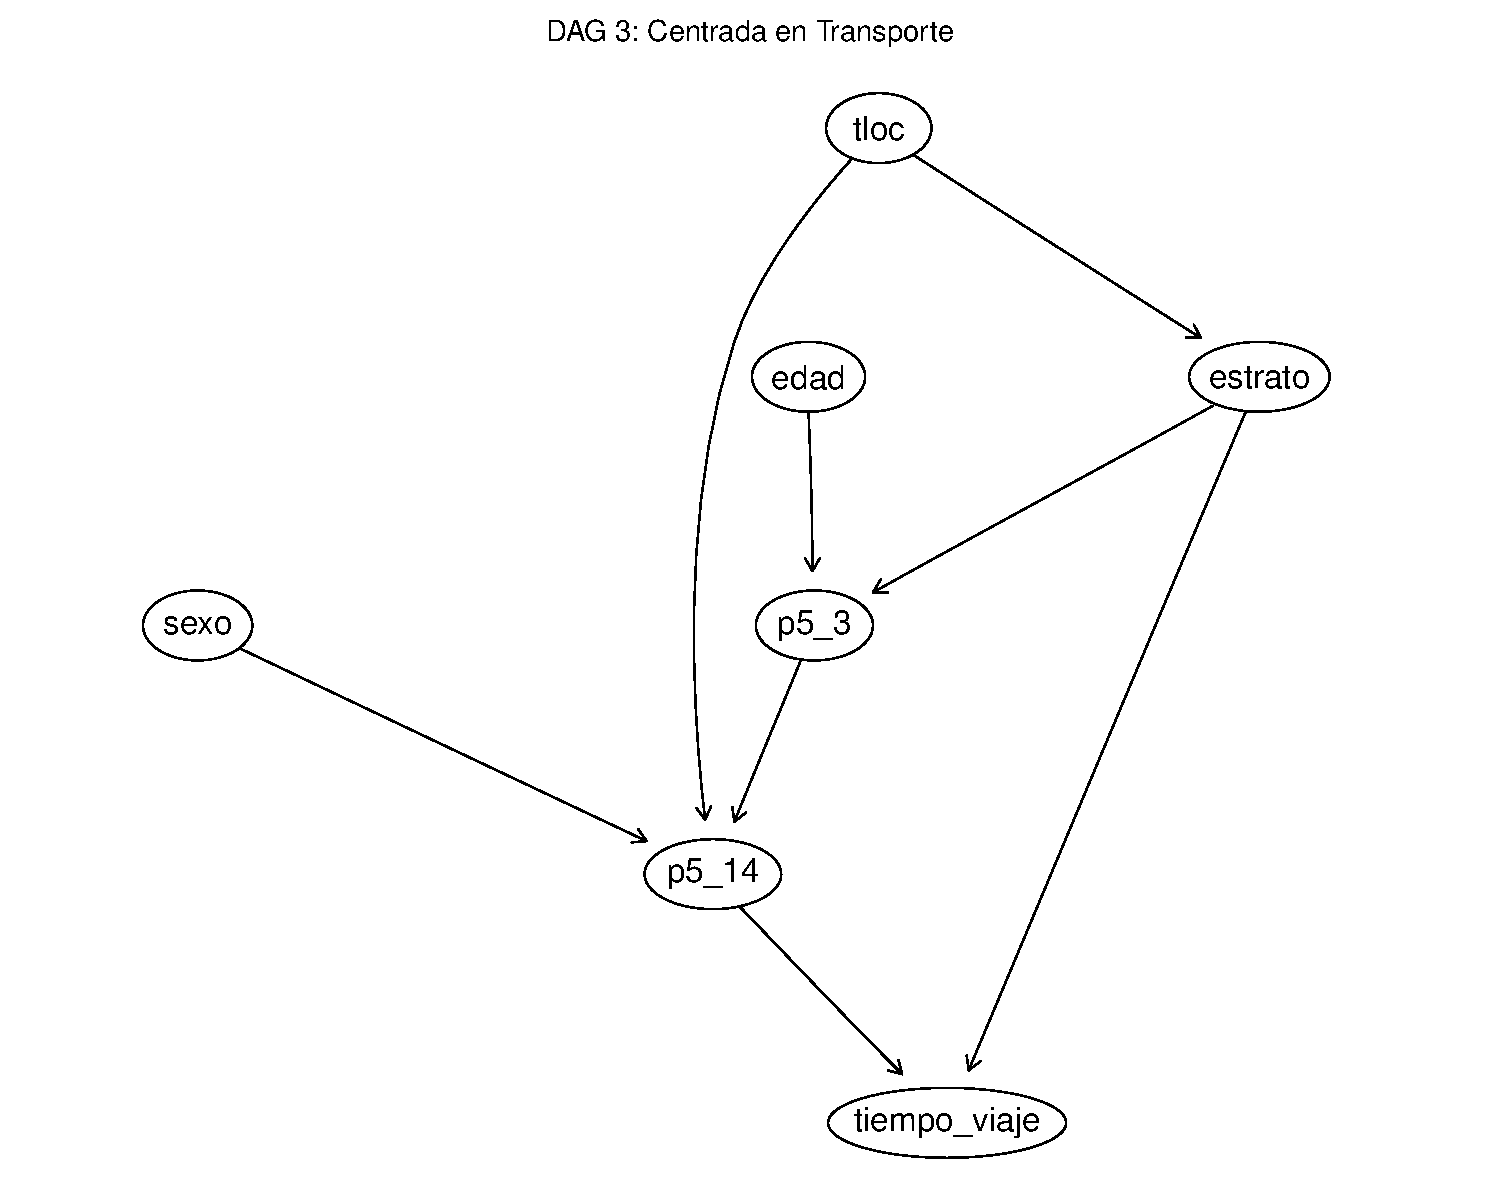
\includegraphics[width=0.8\columnwidth]{figures/DAG3_transporte.pdf}
                \caption{DAG 3: Transporte}
                \label{fig:dag3}
            \end{figure}
            
            $BIC_3=-6419025$
    \end{itemize}
    
    De acuerdo con la métrica $BIC$, la estructura que mejor se ajusta a los datos fue DAG 1, basado en sentido común; seguido por DAG 3, centrada en transporte, y por último, DAG 2, centrada en demografía. Siendo $BIC_1>BIC_3>BIC_2$. 
    
    \item \textbf{DAG óptima}: A través de \textit{Hill-climbing}, algoritmo que maximiza un score dado, se encontró la configuración que mejor se adapta a la estructura de los datos.
    
        \begin{figure}[htbp]
            \centering
            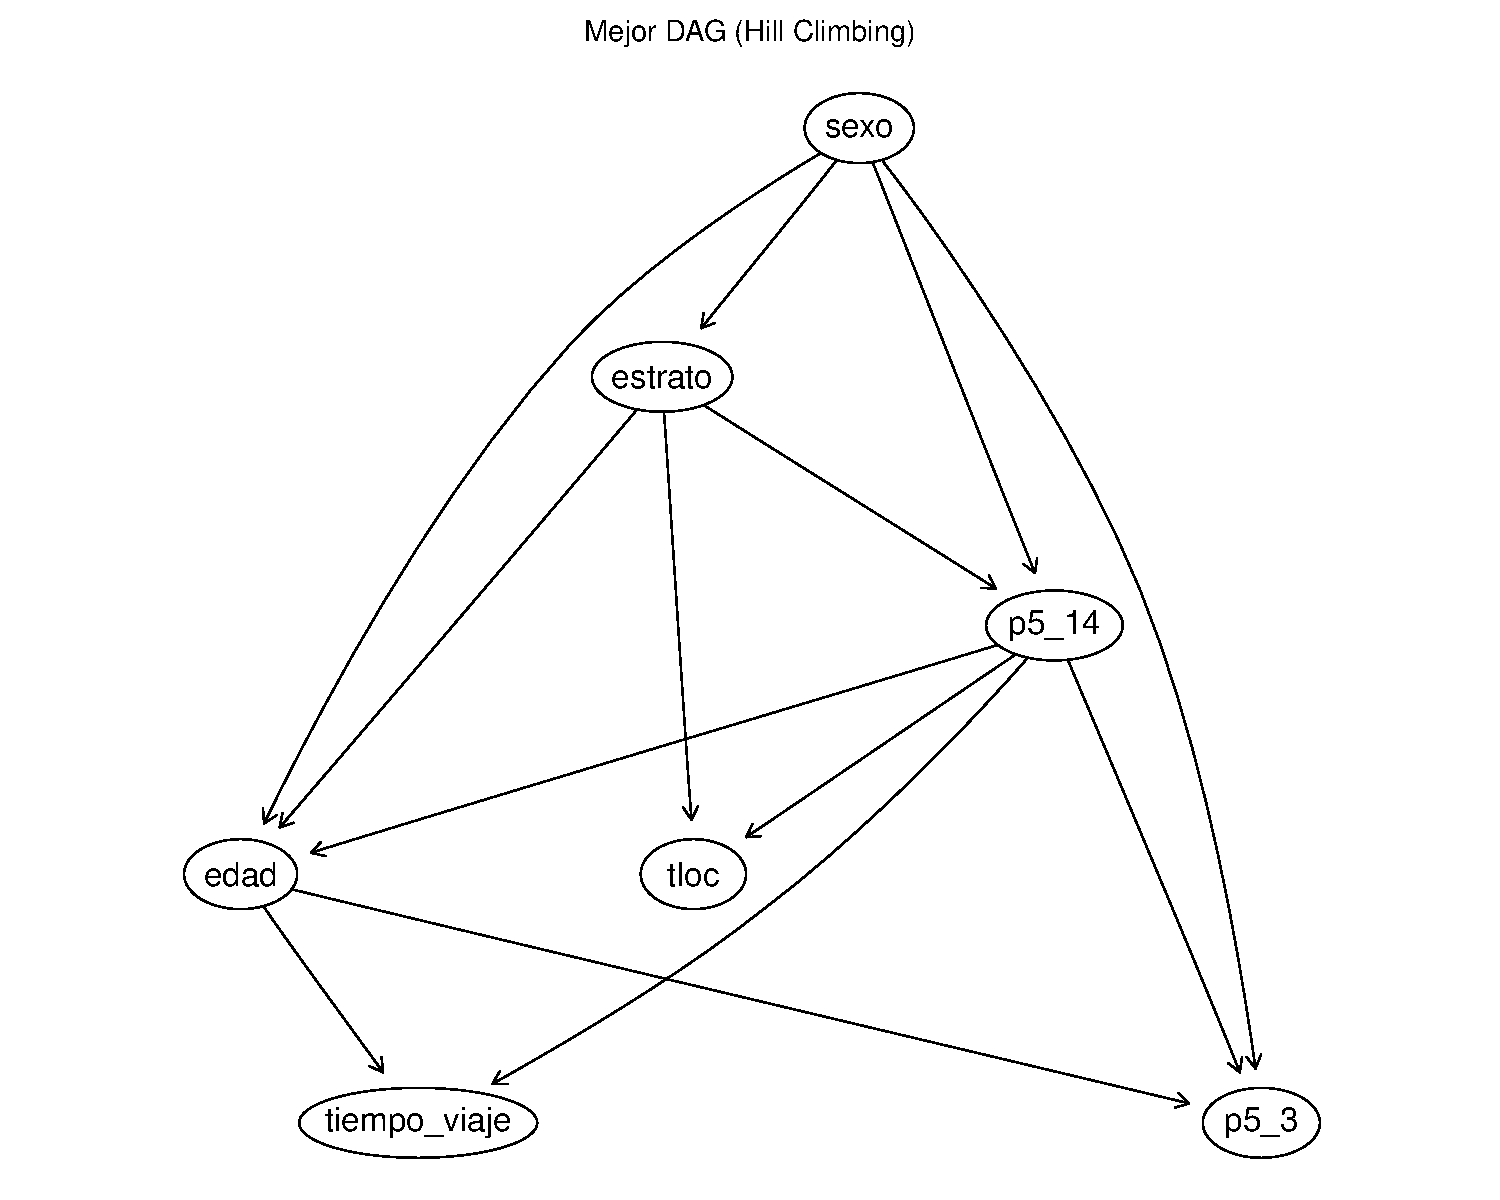
\includegraphics[width=0.8\columnwidth]{figures/DAG_best.pdf}
            \caption{Mejor DAG obtenido por Hill Climbing}
            \label{fig:dag_best}
        \end{figure}

        $BIC_Z=-6152622$
        
        Esta DAG óptima cuenta con un mayor valor en la métrica $BIC$, contra la mejor propuesta anteriormente. Bajo esta estructura se establece la variable \textit{edad} como único nodo independiente, lo que brinda información relevante sobre la alta dependencia de las demás variables respecto a la edad.

        Así mismo se investigó cada relación de dependencia de la DAG óptima, por medio de una Prueba de independencia (condicional). 
        
        
\centering
\begin{tabular}{llr}
\toprule
from & to & strength\\
\midrule
p5\_13 & p5\_6 & 0\\
edad & p5\_13 & 0\\
p5\_3 & p5\_13 & 0\\
p5\_3 & p5\_6 & 0\\
edad & p5\_6 & 0\\
\addlinespace
estrato & tloc & 0\\
sexo & p5\_13 & 0\\
p5\_13 & p5\_14 & 0\\
p5\_14 & estrato & 0\\
sexo & p5\_6 & 0\\
\addlinespace
p5\_14 & tiempo\_viaje & 0\\
edad & p5\_14 & 0\\
sexo & p5\_14 & 0\\
p5\_14 & tloc & 0\\
p5\_6 & estrato & 0\\
\addlinespace
edad & p5\_3 & 0\\
sexo & p5\_3 & 0\\
edad & sexo & 0\\
edad & tiempo\_viaje & 0\\
\bottomrule
\end{tabular}

        
        En la tabla y el heatmap (figura \ref{fig:heatmap_mi}) se aprecia que las dependencias más fuertes son entre \textit{edad} y \textit{sexo}, mientras que varias otras relaciones presentan valores cercanos a cero.
\end{enumerate}

    \begin{figure}[htbp]
        \centering
        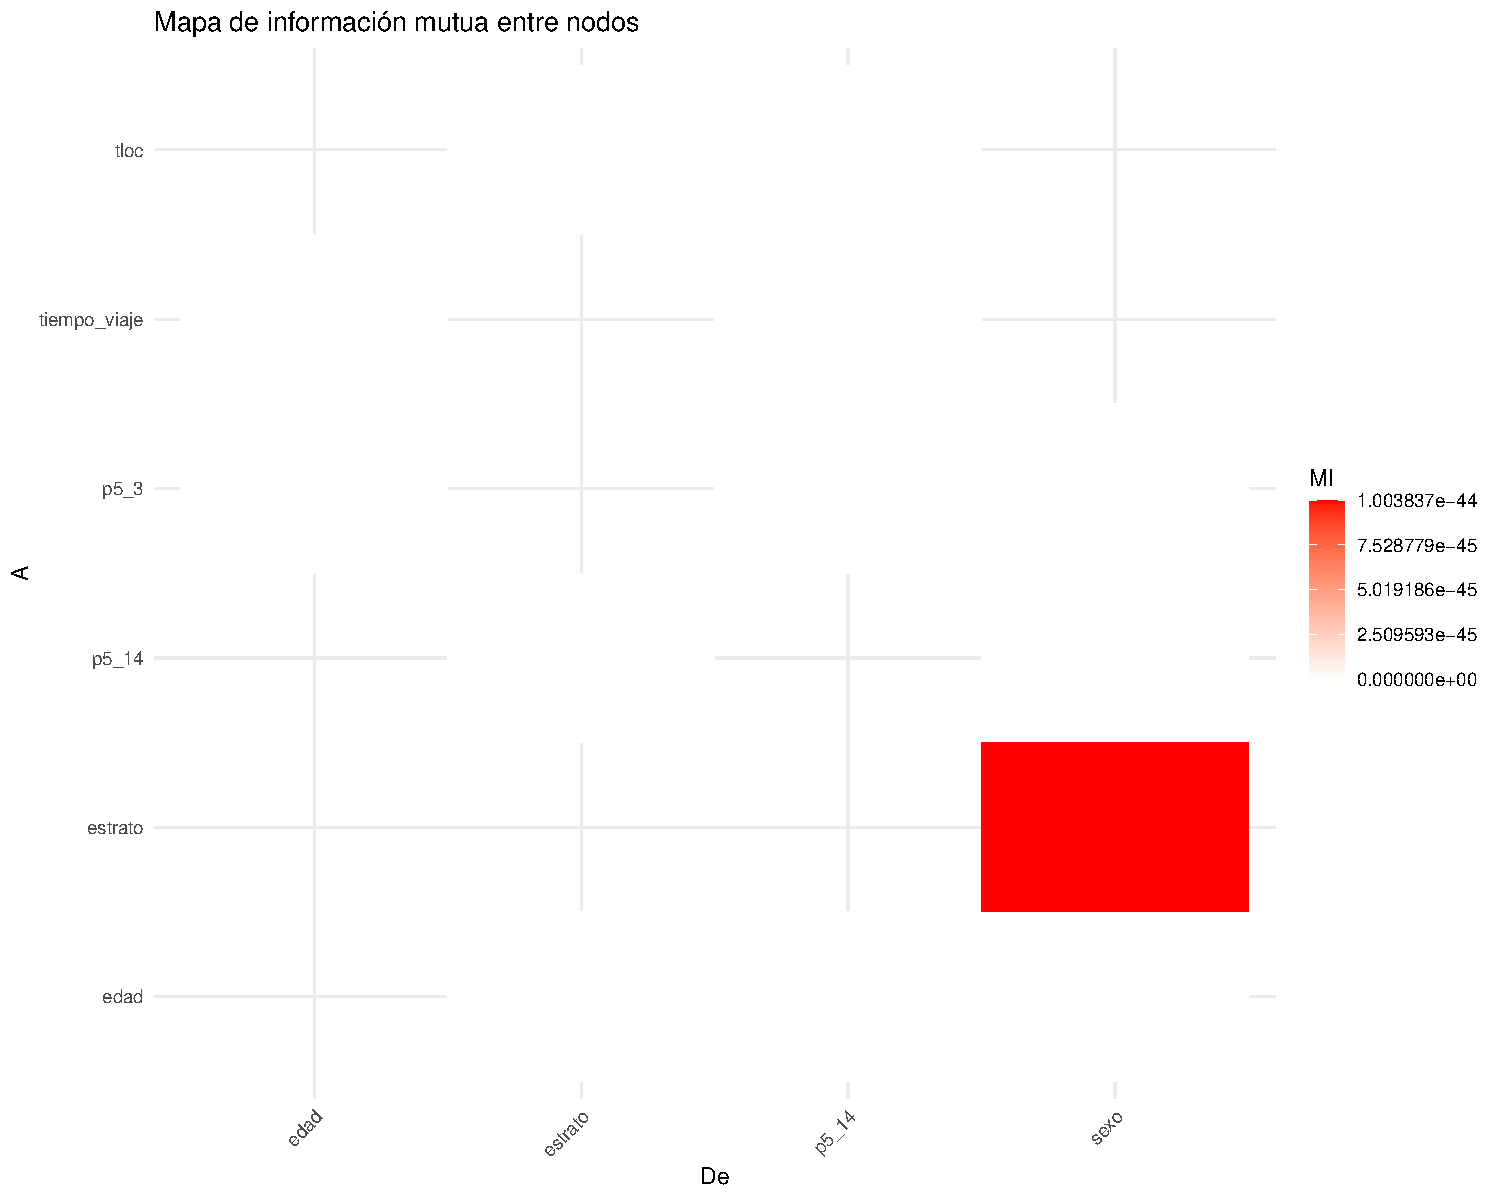
\includegraphics[width=0.8\columnwidth]{figures/heatmap_informacion_mutua.pdf}
        \caption{Heatmap de Información Mutua entre nodos de la red bayesiana}
        \label{fig:heatmap_mi}
    \end{figure}

    
 El hecho de que la fuerza en los arcos sea nula o casi nula implica que las dependencias condicionales entre las variables son demasiado pequeñas o inexistentes en los datos utilizados. Dado que se trabajó conlas variables de interés para dar una respuesta a las queries y se discretizaron las variables usadas de una manera pragmática, esto es indicio de que en la población efectivamente no existe una relación estadística entre las variables o bien que el proceso de limpieza y tratamiento de los datos, así como la eliminacióin de algunos casos con NA redujo la variabilidad disponible en el conjunto de datos. Sin embargo, es posible que con un conjunto de datos donde las categorías de las variables estuvieran más balanceadas se pudieran observar relaciones de dependencia invisibles a los DAGs presentados en este artículo. 
 
\section{Aplicación}
Se realizaron consultas específicas sobre movilidad utilizando la red bayesiana óptima.
\begin{enumerate}
    \item \textbf{¿Cuál es la probabilidad de que una persona mayor de 18 años use como medio de transporte el tren (metro, tren ligero o suburbano)?}  
    {\footnotesize \[
    \mathbb{P}\big(T \in \{\text{metro, tren ligero, suburbano}\} \mid A = \text{adulto}\big) = 0.0868
    \]}
    
    \item \textbf{¿Cuál es la probabilidad de utilizar transporte privado en un día entre semana en comparación con el fin de semana?}  
    {\footnotesize \[
    \mathbb{P}\big(T \in \{\text{automóvil, moto, bicicleta}\} \mid D = \text{semana}\big) = 0.1422
    \]}
    {\footnotesize \[
    \mathbb{P}\big(T \in \{\text{automóvil, moto, bicicleta}\} \mid D = \text{fin de sem}\big) = 0.1603
    \]}
    
    \item \textbf{¿Cuál es la probabilidad de que un hombre adulto use el automóvil por motivos de trabajo?}  
        \[
        \resizebox{0.85\columnwidth}{!}{$
        \mathbb{P}\big(T = \text{automóvil} \mid S = \text{hombre}, A = \text{adulto}, M = \text{trabajo}\big) = 0.1191
        $}
        \]

    
    \item \textbf{¿Quién es más probable que tarde más de 1 hora 30 minutos de casa al trabajo, una persona de estrato bajo o alto?}  
    {\footnotesize
    \[
    \resizebox{\columnwidth}{!}{$
    \mathbb{P}(\text{tiempo de viaje} > 90\ \text{min} \mid E = \text{bajo}, p5\_13 = \text{al trabajo}, p5\_6 = \text{Casa}) = 0.0131
    $}
    \]
    \[
    \resizebox{\columnwidth}{!}{$
    \mathbb{P}(\text{tiempo de viaje} > 90\ \text{min} \mid E = \text{alto}, p5\_13 = \text{al trabajo}, p5\_6 = \text{Casa}) = 0.0170
    $}
    \]
    }

\end{enumerate}

A partir de los resultados obtenidos con la red bayesiana óptima, se pueden destacar los siguientes hallazgos:
\begin{enumerate}
    \item \textbf{Uso de transporte ferroviario en adultos.}  
    La probabilidad de que un adulto utilice transporte ferroviario (metro, tren ligero o suburbano) es de apenas 8.68\%. Esto refleja que, aunque son medios importantes para la movilidad en la ZMVM, su peso relativo dentro de la distribución modal es reducido frente a otros medios de transporte.

    \item \textbf{Diferencia entre semana y fin de semana en transporte privado.}  
    El uso de transporte privado aumenta ligeramente en fines de semana (16.03\%) respecto a los días hábiles (14.22\%). Aunque la diferencia no es muy marcada, indica una mayor preferencia por automóvil y taxi privado en actividades no laborales, como ocio o visitas familiares.

    \item \textbf{Uso del automóvil por hombres adultos en viajes laborales.}  
    La probabilidad de que un hombre adulto utilice automóvil para motivos de trabajo es de 11.91\%. Este valor, relativamente bajo, confirma que gran parte de este grupo recurre al transporte público en sus desplazamientos cotidianos, posiblemente por factores como tráfico, costo de combustible o disponibilidad de estacionamiento.

    \item \textbf{Duración de viajes según estrato socioeconómico.}  
    Las probabilidades de realizar viajes largos (mayores a 90 minutos) de casa al trabajo son bajas en general, aunque ligeramente superiores en el estrato alto (1.70\%) en comparación con el estrato bajo (1.31\%). Esto sugiere que el estrato alto presenta mayor tolerancia a trayectos extensos, probablemente por disponer de transporte privado que facilita recorrer distancias más largas hacia zonas de trabajo, estudio o recreación.
\end{enumerate}
\section{Conclusiones}
En síntesis, estos hallazgos cuantitativos refuerzan la idea de que la movilidad en la ZMVM está condicionada tanto por factores demográficos como socioeconómicos, evidenciando desigualdades en el acceso, uso y experiencia del transporte urbano.
En un futuro se podría buscar realizar un análisis similar al anterior tomando en cuenta más variables y variables más concretas para las incógnitas a responder y quizá sin una discretización tan amplia o con clases mejor balanceadas, con el objetivo de evidenciar relaciones más sutiles entre las variables. Asimismo, sería importante incorporar información extra sobre infraestructura vial o rutas de los servicios de transporte público para enriquecer la interpretación de los resultados y llegar a un modelo que verdaderamente muestre las relaciones de dependencia condicional que seguramente existen entre las variables a emplear.

\section{Referencias}
\begin{thebibliography}{9}
\setlength{\itemsep}{0pt}
\setlength{\parskip}{0pt}
\bibitem{inegi2017} 
Instituto Nacional de Estadística y Geografía (INEGI),
\textit{Encuesta Origen–Destino en Hogares de la Zona Metropolitana del Valle de México 2017},
México, 2018.
Disponible en: \url{https://www.inegi.org.mx/programas/eod/2017/}, consultado el 31 de agosto de 2025.

\bibitem{scutari2025} 
Scutari, M.,
\textit{arc.strength [R package documentation]},
2025.
Disponible en: \url{https://www.bnlearn.com/documentation/man/arc.strength.html}, consultado el 31 de agosto de 2025.

\end{thebibliography}



\end{document}
